\documentclass{article}
\usepackage[english,main=greek]{babel}
\usepackage{geometry}
\usepackage{pgfplots}
\pgfplotsset{width=12cm,compat=1.18}

\newgeometry{vmargin={10mm, 20mm}, hmargin={20mm, 20mm}}

\newcommand{\en}[1]{\foreignlanguage{english}{#1}}

\begin{document}
\title{Εφαρμοσμένα Μαθηματικά Εργαστηριακή Άσκηση 1}
\author{Δημήτριος Γκούμας - \en{cs}04502}
\date{25 Νοεμβρίου 2023}
\maketitle

\begin{itemize}
    \item Διαμέριση \en{$\Delta(J)$}:

    \quad Διαμερίζω το σύνολο \en{$[a, b]$} σε υποδιαστήματα μήκους Δt και πλήθους \en{$(b - a) / \Delta t$}.
    
    \item Διακριτό ανάλογο

    \quad Από την μέθοδο \en{Euler} προκύπτει το διακριτό ανάλογο: 
    \en{\[y(t) = y(t - 1) + \Delta t * f(t, y(t))\]}

    \quad{Στο πρόβλημα 2 όπου \en{$f(t, y(t)) = y(t)$} το διακριτό ανάλογο γίνεται:
    \en{\[y(t) = y(t-1) / (1 - \Delta t)\]}}
    
    \item Αλγόριθμος

    \quad Ο αλγόριθμος είναι παρόμοιος και για τα 2 προβλήματα της άσκησης.

    \begin{enumerate}
        \item Ζητούνται από τον χρήστη τα \en{$a, b, y_0, \Delta t$}.
        \item Υπολογίζονται τα βήματα ως \en{$steps = (b - a) / \Delta t$}.
        \item Αρχικοποιείται το \en{array} \en{$results$} με μέγεθος \en{$steps$}.
        \item Η αναδρομική συνάρτηση έχει τον εξής αλγόριθμο:
        
        \begin{itemize}
            \item Δέχεται ως παράμετρους τα \en{$y_0, \Delta t, steps, results$}.
            \item \en{(Base case)} Ελέγχεται αν έχει φτάσει στο τελευταίο βήμα (όταν \en{$steps = 0$}).
            \item Εάν όχι, συνεχίζεται η αναδρομή χρησιμοποιόντας το \en{$y(i-1)$} για να υπολογιστεί το \en{$y(i)$}.
            \item Εάν ναι, επιστρέφεται το \en{$y(i)$} χρησιμοποιόντας το \en{$y_0$} για να το υπολογίσει.
            \item Σε όλη τη διάρκεια της αναδρομής, το \en{$y(i)$} αποθηκεύεται στο \en{$results[i]$}.
        \end{itemize}

        \item Εκτύπωση των αποτελεσμάτων.
    \end{enumerate}
\end{itemize}



\clearpage



\begin{table}
    \centering
    \begin{tabular}{|c|c|c|c|c|c|c|}

    \hline 
     & \multicolumn{3}{|c|}{\en{$\Delta t = 0.2$}} & \multicolumn{3}{|c|}{\en{$\Delta t = 0.1$}} \\

    \hline
    \en{$t_i$} & \en{$y(t_i)$} & \en{$y_i$} & \en{$e_i = | y(t_i) - y_i |$} & \en{$y(t_i)$} & \en{$y_i$} & \en{$e_i = | y(t_i) - y_i |$} \\

    \hline
    0.0 & 1.000 & 1.000 & 0.000 & 1.000 & 1.000 & 0.000 \\
    0.1 & 1.105 & -     & -     & 1.105 & 1.111 & 0.006 \\
    0.2 & 1.221 & 1.250 & 0.029 & 1.221 & 1.234 & 0.013 \\
    0.3 & 1.349 & -     & -     & 1.349 & 1.371 & 0.022 \\
    0.4 & 1.491 & 1.562 & 0.071 & 1.491 & 1.524 & 0.033 \\
    0.5 & 1.648 & -     & -     & 1.648 & 1.693 & 0.045 \\
    0.6 & 1.822 & 1.953 & 0.131 & 1.822 & 1.881 & 0.059 \\
    0.7 & 2.013 & -     & -     & 2.013 & 2.090 & 0.077 \\
    0.8 & 2.225 & 2.441 & 0.216 & 2.225 & 2.323 & 0.098 \\
    0.9 & 2.459 & -     & -     & 2.459 & 2.581 & 0.122 \\
    1.0 & 2.718 & 3.051 & 0.333 & 2.718 & 2.867 & 0.149 \\
    \hline

    \end{tabular}
    \caption{Πρόβλημα 1}
\end{table}


\begin{table}
    \centering
    \begin{tabular}{|c|c|c|c|c|c|c|}

    \hline 
     & \multicolumn{3}{|c|}{\en{$\Delta t = 0.2$}} & \multicolumn{3}{|c|}{\en{$\Delta t = 0.1$}} \\

    \hline
    \en{$t_i$} & \en{$y(t_i)$} & \en{$y_i$} & \en{$e_i = | y(t_i) - y_i |$} & \en{$y(t_i)$} & \en{$y_i$} & \en{$e_i = | y(t_i) - y_i |$} \\

    \hline
    0.0 & 0.000  & 0.000 & 0.000 & 0.000  & 0.000 & 0.000 \\
    0.1 & 0.579  & -     & -     & 0.579  & 0.600 & 0.021 \\
    0.2 & 1.041  & 1.200 & 0.159 & 1.041  & 1.138 & 0.097 \\
    0.3 & 1.297  & -     & -     & 1.297  & 1.508 & 0.211 \\
    0.4 & 1.309  & 1.940 & 0.631 & 1.309  & 1.644 & 0.335 \\
    0.5 & 1.098  & -     & -     & 1.098  & 1.536 & 0.438 \\
    0.6 & 0.741  & 1.724 & 0.983 & 0.741  & 1.235 & 0.494 \\
    0.7 & 0.349  & -     & -     & 0.349  & 0.840 & 0.491 \\
    0.8 & 0.043  & 0.934 & 0.891 & 0.043  & 0.472 & 0.429 \\
    0.9 & -0.077 & -     & -     & -0.077 & 0.245 & 0.322 \\
    1.0 & 0.041  & 0.480 & 0.439 & 0.041  & 0.240 & 0.199 \\
    1.1 & 0.394  & -     & -     & 0.394  & 0.482 & 0.088 \\
    1.2 & 0.920  & 0.964 & 0.044 & 0.920  & 0.936 & 0.016 \\
    1.3 & 1.515  & -     & -     & 1.515  & 1.516 & 0.001 \\
    1.4 & 2.056  & 2.124 & 0.068 & 2.056  & 2.104 & 0.048 \\
    1.5 & 2.437  & -     & -     & 2.437  & 2.581 & 0.144 \\
    1.6 & 2.589  & 3.078 & 0.489 & 2.589  & 2.855 & 0.266 \\
    1.7 & 2.498  & -     & -     & 2.498  & 2.882 & 0.384 \\
    1.8 & 2.212  & 3.133 & 0.921 & 2.212  & 2.681 & 0.469 \\
    1.9 & 1.824  & -     & -     & 1.824  & 2.325 & 0.501 \\
    2.0 & 1.455  & 2.421 & 0.966 & 1.455  & 1.927 & 0.472 \\
    \hline

    \end{tabular}
    \caption{Πρόβλημα 2}
\end{table}



\clearpage



\begin{center}
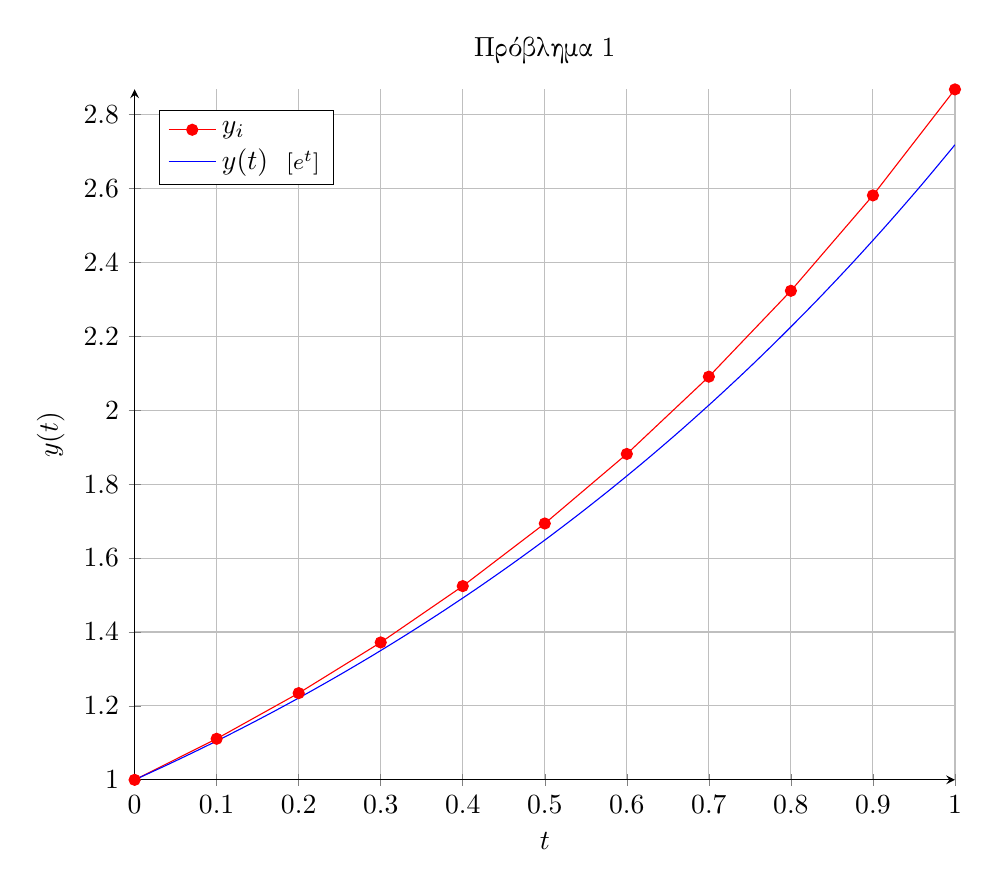
\begin{tikzpicture}
\begin{axis}[
    axis lines = left,
    xlabel = $t$,
    ylabel = $y(t)$,
    title={Πρόβλημα 1},
    grid=major,
    legend cell align={left},
    legend pos=north west,
]

\addplot [
    color=red,
    mark=*,
] coordinates {
    (0, 1)
    (0.1, 1.111111)
    (0.2, 1.234568)
    (0.3, 1.371742)
    (0.4, 1.524158)
    (0.5, 1.693509)
    (0.6, 1.881676)
    (0.7, 2.090752)
    (0.8, 2.323057)
    (0.9, 2.581175)
    (1, 2.867972)
};

\addlegendentry{$y_i$}

\addplot [
    color=blue,
    domain=0:1,
    smooth
] {exp(x)};

\addlegendentry{$y(t)$ \space {\footnotesize [$e^t$]}}

\end{axis}
\end{tikzpicture}
\end{center}



\begin{center}
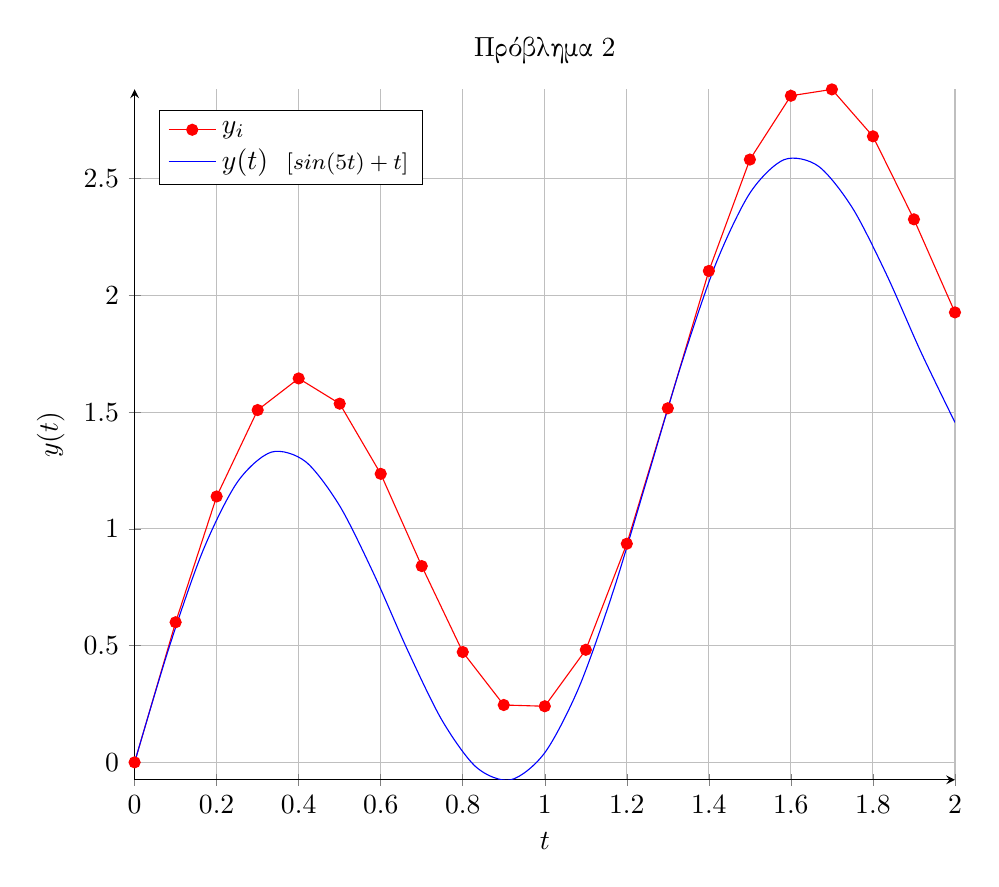
\begin{tikzpicture}
\begin{axis}[
    axis lines = left,
    xlabel = $t$,
    ylabel = $y(t)$,
    title={Πρόβλημα 2},
    grid=major,
    legend cell align={left},
    legend pos=north west,
]

\addplot [
    color=red,
    mark=*,
] coordinates {
    (0, 0)
    (0.1, 0.6)
    (0.2, 1.138791)
    (0.3, 1.508942)
    (0.4, 1.644311)
    (0.5, 1.536238)
    (0.6, 1.235666)
    (0.7, 0.840670)
    (0.8, 0.472441)
    (0.9, 0.245619)
    (1, 0.240222)
    (1.1, 0.482053)
    (1.2, 0.936387)
    (1.3, 1.516473)
    (1.4, 2.104766)
    (1.5, 2.581718)
    (1.6, 2.855035)
    (1.7, 2.882285)
    (1.8, 2.681279)
    (1.9, 2.325714)
    (2, 1.927128)
};

\addlegendentry{$y_i$}

\addplot [
    color=blue,
    domain=0:2,
    smooth,
] {sin(deg(5*x)) + x};

\addlegendentry{$y(t)$ \space {\footnotesize [$sin(5t) + t$]}}

\end{axis}
\end{tikzpicture}
\end{center}



\end{document}